\documentclass[prl,aps,epsf,showpacs,twocolumn,letterpaper]{revtex4}
\usepackage[T1]{fontenc}
\usepackage{newtxtext, newtxmath}
\usepackage{graphicx}
\usepackage{float}
\usepackage{latexsym,amsmath,amssymb,bm,euscript,braket}
\usepackage{color}
\usepackage{subfigure}
\usepackage{epstopdf}
\usepackage[colorlinks=true,linkcolor=blue,citecolor=blue]{hyperref}
\usepackage{hyperref}

%%%%%%%%%%%%%%%%%%%%%%%%%%%%%%%%%%%%%%%%
% FOR MAC'S PERSONAL USE WITH "chktex" %
%%%%%%%%%%%%%%%%%%%%%%%%%%%%%%%%%%%%%%%%
% spaces after commands
% chktex-file 1
% spaces before '('
% chktex-file 36

%%%%%%%%%%%%%%%%%%%%%%%%%%%%%%%%%%%%
% Automatic numbering for sections %
%%%%%%%%%%%%%%%%%%%%%%%%%%%%%%%%%%%%
\let\oldsection\section
\renewcommand{\section}[1]{\stepcounter{section}\oldsection{\Roman{section}. #1}}

%%%%%%%%%%%%%%%%%%%%%%%%%%%%%
% Define the trace operator %
%%%%%%%%%%%%%%%%%%%%%%%%%%%%%
\DeclareMathOperator{\tr}{Tr}

\newcommand{\oim}[1]{{\color{red}$\clubsuit$ #1}}

\bibliographystyle{apsrmp}

\begin{document}



\title{Many-Body Localization in Spin Chain System with Quasi-Periodic Disorder}
\author{Mac Lee, Thomas R. Look, S. P. Lim and D. N. Sheng}

\affiliation{Department of Physics and Astronomy, California State University,
Northridge, California 91330, USA}


\begin{abstract} 


\end{abstract}

\pacs{73.40.Hm, 71.30.+h, 73.20.Jc }
\maketitle


\section{Introduction}

The interplay of random disorder and many-body interactions has attracted a lot 
of recent research activity\cite{basko2006, oganesyan2007, pal2010, 
znidaric2008, huse2013, nandkishore2015, altman2015, huse2014, nandkishore2014, 
pekker_hilbert2014}.  The many-body localized (MBL) quantum 
phase\cite{nandkishore2015, altman2015, huse2014, nandkishore2014, 
pekker_hilbert2014} of matter is distinctly different from both Anderson 
localization in non-interacting systems and the ergodic (thermal) phase for 
interacting systems with weaker disorder.  The ergodic phase follows the 
eigenstate thermalization hypothesis (ETH) which describes how an isolated 
self-interacting quantum system can thermalize under its own internal dynamics 
in agreement with quantum statistical mechanics\cite{deutsch1991, 
srednicki1994, rigol2008}.  A system in the MBL phase, on the other hand, fails 
to thermalize even for its highly excited eigenstates on any time scale, 
resulting in new statistics for such systems\cite{basko2006, oganesyan2007, 
pal2010, znidaric2008, huse2013, nandkishore2015, altman2015, huse2014, 
nandkishore2014, pekker_hilbert2014}.  Many remarkable properties of an MBL 
phase have been established\cite{nandkishore2015, altman2015, huse2013, 
nandkishore2014, oganesyan2007, pal2010, znidaric2008, rigol2008, serbyn2014, 
kwasigroch2014, yao2014, vasseur2015, huse2014, serbyn2013, ros2015, 
chandran2014, grover2014, agarwal2015, knap2015, luitz2015, devakul2015, 
torres2015, canovi2011, cuevas2012, bauer2013, kjall2014, luca2013, iyer2013, 
pekker_hilbert2014, johri2014, bardarson2012, andraschko2014, laumann2014, 
hickey2014, nanduri2014, barlev2014, imbrie2014, groverf2014, ponte2015, 
huang2015, you2015, serbyn2015, singh2015, barlev2015, deng2015, chen2015} 
based on extensive theoretical studies.  The existence of both the ergodic and 
MBL phase suggests a dynamic quantum phase transition between 
them\cite{basko2006, pal2010, oganesyan2007, kjall2014, vosk_theory2014, 
potter2015trans, serbyn2015, agarwal2015, knap2015, lim2016, zhang2016, 
zhang2016a, yu2016, vedika2016, dumitrescu2017}.  Random disorder introduces 
rare Griffiths regions\cite{vosk_theory2014, potter2015trans, 
knap2015,luitz2015,lim2016} which may have singular contributions in driving 
such a phase transition, but there is still limited quantitative understanding 
about their effects\cite{vedika2017}.  Most numerical studies of the MBL 
transition have focused on random disorder models for spin chains\cite{pal2010, 
kjall2014, luitz2015, yu2016, vedika2016}, while very recently the dynamic 
quantum phase transition has been analyzed with a close comparison between the 
quasi-periodic and random disorder models, which point to the possibility of 
two universality classes for the quantum phase transition\cite{vedika2017, 
vedika2016}.

Time evolution of many-body systems has been studied for spin-chains with a 
randomly distributed field\cite{kjall2014,luitz2016time}, which can be used to 
address the dynamics of the thermal to MBL phase 
transition\cite{nandkishore2015,vosk_theory2014,potter2015}.  After a global 
quantum quench, power-law growth of bipartite entanglement entropy is observed 
for thermal states while logarithmic growth is observed for MBL states where 
the local memory of an initial product state remains at infinite 
time\cite{luitz2016time}.


In this paper we report eigenstate and time-dependent studies of spin chains 
with quasi-periodic disorder.  Through exact diagonalization (ED) studies, we 
find a dynamic quantum phase transition from the ergodic phase to the MBL phase 
that is similar to spin chains with random disorder.  However, systems with 
quasi-periodic disorder appear to be more efficient at localizing which is 
demonstrated by a smaller critical disorder, $W_c \sim 2$, compared to systems 
with random disorder.  We also performed time-evolution of randomly selected 
product states and studied their entanglement entropy, imbalance and spin glass 
order. Similar to the random field model, we find both power-law and 
logarithmic growth of the entanglement entropy and that these two regimes are 
demarcated by $W_c$, the boundary between the ergodic and MBL phases.  In 
addition to the general growth trends, we also notice pseudo-periodic 
oscillations in our entropy plots for small $t$'s. The imbalance and spin glass 
order also display markedly different behaviors in the two different phases 
under time evolution, albeit in a different manner from that of entanglement 
entropy. In the thermal phase, both imbalance and spin glass order decay to a 
saturation level rather rapidly; in the MBL phase, on the other hand, both 
imbalance and spin glass order hover around their respective initial values for 
extremely long times, indicating the system is frozen in place and does not 
follow descriptions of quantum statistical mechanics. These results show that 
quasi-periodic spin chains show qualitatively similar behaviors with random 
spin chains with these standard observables.


\section{Model and identify the ergodic to many-body localized phase transition}


We study the Heisenberg spin-1/2 chain with the following Hamiltonian:
\[
  H = J\sum_{i=1}^{N-1} \mathbf{S}_i \cdot \mathbf{S}_{i+1}
  + \sum_{i}^{N} W\cos(2\pi c i+\phi) S_i^z \text{.}
\]
In this Hamiltonian, $\mathbf{S}_i$ is the total spin operator for site $i$ and
$J$ is the nearest neighbor coupling constant.
For the second term of the Hamiltonian which describes the coupling between the
$z$-directional field and our sites, $W$ is the scaling factor of the field
strength and $\phi$ is the phase factor of the cosine function that governs the
field.
Both parameters are adjusted as we study their effects on the behavior of the
system.
The remaining parameter, $c$, is an irrational number which, for the course of
our study, is fixed at $\sqrt{2} - 1$.


This model is similar to the one studied recently in Ref.\cite{vedika2016}.
In this paper, however, we will place our focus on the time-evolution of the
states, which have not been thoroughly studied for systems with quasi-periodic
potentials.
For all our calculations, we used open-boundary condition since it allows a
larger window for observing the time evolution of physical
quantities\cite{luitz2016time} before they saturate due to finite-size effects.
All the results are obtained with highly excited states with energies near the
center of the spectrum.


\begin{figure}
  \includegraphics[angle=-90,width=0.9\linewidth]{entropy_plot.ps} \\
  \includegraphics[angle=-90,width=0.9\linewidth]{dispersion_plot.ps} \\
  \caption{(Color online) (a) For system sizes $L = 10-16$, we notice a crossing
    of $W$ at approximately $1.6$, indicating a quantum phase change.
    As we can see, the dispersion of $\braket{Sz}$ decays as $W$ increases and
    tends to zero at larger values of $W$.
    We conclude that this corroborates our conclusion from the entropy plot that
    the many-body system freezes and fails to thermalize with increasing
    disorder strength.
    (b) For system sizes $L = 10-16$, we notice the bipartite entanglement
    entropy of the many-body system decays as $W$ increases.
    We conclude from our plot that the entropy of a system described by our
    model tends to zero at high disorder strength.
    We also notice that our graphs cross at around $W_c=1.6$, indicating a
    quantum phase transition at that point.
  }
\label{fig1}
\end{figure}
\begin{figure}[b]
  \includegraphics[angle=-90, origin=c,  width=3.4in]{newfig1a.ps}\\
  \vspace{-0.6in}
  \includegraphics[angle=-90,width=3.1in]{newfig1b.ps}\\
  \vspace{0.1in}
  \caption{(Color online) (a) Entropy $S(t)$ of a $L=16$ system as a function of
    time for $W < W_c$.
    We can see a power-law growth of the entanglement entropy in the logarithmic
    plot.
    (b) $S(t)$ of the same system with $W > W_c$. Notice the logarithmic time
    dependence.
  }
\label{fig2}
\end{figure}

\begin{figure}[b]
  \includegraphics[angle=-90,width=3.2in]{newfig1c.ps}\\
  \vspace{-0.10in}
  \includegraphics[angle=-90,width=3.2in]{newfig1d.ps}\\
  \hspace{0.0in}
  \vspace{-0.3in}
  \includegraphics[angle=-90,width=3.2in]{newfig1e.ps}\\
  \vspace{0.12in}
  \caption{(Color online) (a) 
    For system sizes ranging from $12$ to $20$, at $W=1$, we observe the
    entanglement entropy increases rapidly until $t \sim 1$.
    At $1<t<50$, all the $S(t)$ data could be fitted into a straight line.
    For bigger $t$, we see that $S(t)$ saturates to $\frac{L}{2} \ln{2}$,
    consistent with the thermal entropy of the ergodic phase.
    (b) At $W=2$, for smaller system sizes, we observe that $S(t)$ grows slower
    than it is predicted by the power law; on the other hand, $L=20$ behaves as
    expected and the growth of its entropy over time follows the power law.
    (c) At $W=3$, we notice that all $S(t)$ plots fit to a straight line in the
    log-linear plot, indicating logarithmic growth.
  }
\label{fig3}
\end{figure}


\begin{figure}[b]
  \includegraphics[angle=-90,width=3.in]{newfig2a.ps}\\
  \vspace{-0.0in}
  \includegraphics[angle=-90,width=3.in]{newfig2b.ps}\\
  \hspace{0.0in}
  \vspace{-0.in}
  \caption{(Color online) (a) Imbalance $I(t)$ for a $L=16$ system with $1 < W <
    4$.
    At small values of $W$, we notice the imbalance of the system decays
    rapidly; however, when $W$ is increased beyond $W_c = 1.6$, we notice the
    imbalance ceases decaying and remains at a certain level.
    This is consistent with the MBL behavior where the initial values of the
    local observables for each site $i$ is preserved.
    (b) Spin glass order as defined in eq.\ref{eq:sgo}.
    At small values of $W$, correlations between spins are short ranged and
    $\chi(t)$ decays to $1$ over time; at large values of
    $W$, $\chi(t)$ remains close to its initial value even at very long time,
    further corroborating our assertion of a quantum phase transition.
  }
\label{fig4}
\end{figure}


\begin{figure}[b]
  \includegraphics[angle=-90,width=0.92\linewidth]{newfig3a.ps} \\
  \includegraphics[angle=-90,width=0.92\linewidth]{newfig3b.ps} \\
  \caption{(Color online) (a)
    \bf Needs to be written
  }
\label{fig5}
\end{figure} 


We  perform Lanczos exact diagonalization (ED) calculations   to obtain  energy
eigenstates around  the energy $E$ at a target  energy  density $\varepsilon$
for  systems with different  number of sites $L=10-16$  in the total $S_z=0$
sector.  Specifically, for each disorder configuration, we first calculate the
ground state energy  $E_0$ and the maximum energy $E_\text{max}$, which are used
to define the target energy density $\varepsilon = (E-E_0)/(E_\text{max} -E_0)$.
%Physical quantities\cite{luitz2015}  including the bipartite entanglement
%entropy,  energy level statistics and bipartite  fluctuation of the subsystem
%magnetization are obtained and averaged over disorder configurations and
%sometimes also averaged over  30 energy eigenstates with energies closest to
%the given energy density $\varepsilon$ as detailed below.
We first determine the localization of the MBL transition based on the
entanglement entropy and the fluctuations of the half-system
magnetization\cite{luitz2015}.  The Von Neumann entanglement entropy of the
system  $S$ is obtained  from all eigenvalues of the reduced density matrix
$\rho_A$ as $S=- \tr \rho_A \ln \rho_A$, by partitioning the system in  the
middle.  The entropy is averaged over 30 ($L=12$) to 200 ($L=16$) eigen states
near energy density $\varepsilon=0.5$ in the middle of all eigenstates,   and
$1000$ disorder configurations by choosing random $\phi$ between $(0, 2\pi)$.
As shown in  Fig. 1(a), we plot the  ratio of  entanglement entropy over the
number of system sites  $S/L$ for  different systems  from $L=10$ to $16$  at
the energy density $\varepsilon =0.5$ as a function of random field strength
$W$.  On the  small $W$ side, we have seen an increase of the $S/L$ with $L$,
which saturatue to the Page value ($S/L \sim 0.5\ln(2)$ for large $L$ limit)
following the volume law of the ergodic phase.    On the  larger $W$ side, $S/L$
approaches zero indicating the area law  entanglement and non-ergodic behavior
where the MBL state is realized.  With varying $W$,  all data points
approximately cross each other around  a critical value  $W_c \sim 1.6$.  We
compare the entanglement entropy behavior with the  bipartite fluctuations $F$
of the subsystem magnetization $S^z_A$~\cite{luitz2015,song2012}, which is
defined as $F=\braket{{S^{z}_A}^2} - \braket{S^z_A}^2$ as shown  in Fig. 1(b).
We see that the $F/N$ increases on the  small  $W$ side, while it becomes
vanishing small on the larger $W$ side.  The $F/N$ curves for different $N$
approximately cross each other around the critical field strength $W_c=1.6$ in
consistent with the behavior of the entanglement entropy.  In fact, we see that
there is an approximate proportional relations between $S$ and $F$  for all $W$
region. 




We further use the  level statistics analysis from the random matrix
theory\cite{atas2013,oganesyan2007} to probe the localization-delocalization
characteristics of  energy  eigenstates.
%In the delocalized  regime, the level-spacing  distribution is described by the
%Gaussian orthogonal ensemble (GOE) statistics, which represents extended levels
%with level-repulsion  between them because of the overlap of  energy
%eigenstates in real space.  In the localized regime, the level-spacing
%distribution  is determined by Poisson statistics as  wave-functions close in
%energy are exponentially localized with no level repulsion between
%them\cite{mehta1991}.
In the energy spectrum analysis\cite{luitz2015}, we define the adjacent  energy
gap $\delta_n=E_n-E_{n-1}$ as the energy difference between the $n$-th and
$(n-1)$-th eigenstates, then the adjacent gap ratio can be defined as
$r_n=\min(\delta_n, \delta_{n+1})/\max(\delta_n, \delta_{n+1})$.  We  average the
gap ratio $r=\langle r_n\rangle$  over $30-200$  states near the spectrum center at
$\varepsilon=0.5$   and more than 1000 random  potential configurations for each
given disorder  strength $W$.   As shown in Fig. 1(c),   we see that at the
small $W$ side, $r$ approaches  the Gaussian  orthogonal ensemble  value
(0.5307),  which represents extended levels with level-repulsion  between them
because of the overlap of  energy eigenstates in real space.  On the stronger
$W$ side,  $r$ reaches the Poisson value $(2\ln2-1\simeq 0.3863)$ for larger
systems representing the level statistics of   localized states, where  states
close in energies are  exponentially localized with exponential small overlap
without level repulsion between them\cite{mehta1991}.  A similar level crossing
for all curves is also seen in Fig.1(c),  indicating the same critical point for
the dynamic quantum phase transition.  We also note that,   the critical point
we determined representing an lower  bound for the transition as the crossing
points between larger $L$ curves are moving towards larger $W$ side.    This
feature was also observed in a diferent model for quasi-periodic
systems\cite{vedika2016}.




\subsection{Time-Evolution of quantum state}

We study the quantum dynamics of the quasi-periodic systems after a global
quantum quench.  Here,  we start from a product state
$\ket{\Psi(0)}=\ket{\sigma_1, \sigma_2, \ldots , \sigma_L}$  at the time $t=0$
after the quench, where $\sigma_i=\pm$ represents  the spin-z component $\pm
1/2$ at site $i$.  The state at time $t$ can be obtained as $\ket{\Psi(t)} =
e^{-iHt}\ket{\psi(0)}=e^{-iH\Delta t}\ket{\psi(t-\Delta t)}$ (with setting $\hbar=1$).
We calculate the time evolution of an initial  state  based on  a projection of
the Hamiltonian to the Krylov space spanned by
$\ket{\Psi_0}$, $H\ket{i\Psi_0}$, \ldots, $H^n\ket{\Psi_0}$  using the Lanczos
algorithm by calculating all eigenstates in this space to obtain the
time-evolution operator\cite{luitz2015}.  Using a reasonalble small time step
$\delta t \sim 0.2/J$ allows high accurate results with a small $n=30-60$.


We first discuss the general behavior of the  entanglement entropy as a function
of time as shown in Fig. 2.  On the small $W$ side shown in Fig. 2(a),  we find
that the entropy $S(t)$ grows power-lawly with time $t$ before it reaches the
saturated value $\frac L 2 \ln2$ at long time limit.  On the larger  $W$ side,
we find a much slower growth, which can be fit with a logrithmic growing
function as shown in Fig. 2(b) for $W=3-5$.  


Now we analyze the finite-size scaling behavior of the $S(t)$.  For small $W=1$
as shown in Fig. 3(a),  we find that the initial expansion ($t\sim 1$) of the
$S(t)$ is exponential and system size independent.  For the intermediate time
regime,  the $S(t)$ expands powerlawly until the finite-size effect sets in.
With the increase of $L$,  we find winder time interval for the powerlaw growth
of  the $S(t)$.  Interestingly,  very similar behavior and a smaller window of
the powerlaw growing $S(t)$ are found for $W=2$.  The powerlaw growth indicated
by the straight line in the Fig.3(b) is most clear for larger system size
$N=20$.  This is a strong indication that the $W=2$  is in the thermal phase
consistent with the moving of the crossing point toward larger $W$ with the
increase of $N$ observed in Fig. 1.  We further look into the $S(t)$  at  a
larger $W=3$.  Here we observe that for  small $t$,  $S(t)$ expands
exponentially from the product state to a superposition state for $t\sim 1$,
which then followed by oscillating of $S(t)$.  With further increase of $t$,  we
observe a logrithmic growth of $S(t)$ for time range more than two orders of
magnitude.  The range of $t$ for the logrithmic growing  of $S(t)$ becomes
larger with the increase of $W$.   These results confirm the MBL phase with
similar behavior as the random field case as studied before by Luitz et.
al\cite{luitz2015}. 


Now we address the time evolution of the spin correlations.  As we start from
the product state $|\Psi(0)>$ where the spin-z on each site is  $\pm 1/2$  while
the total $S_z$ of all sites are zero. We define the following time correlators
for spin-z  as 
\begin{equation}
  I(t)=\frac{4}{L} \sum_{j=1}^L \braket{\Psi(0)|S_j^z(0)S_j^z(t)|\Psi(0)}
  \text{,} \label{eq:imb}
\end{equation}
which detects the  total imbalance of
spin-z. As shown in Fig.4(a),  we find a systematic changes of the properties of
the $I(t)$ as $W$ is varied.   For smaller $W=1$,  we see that the long time
behavior of the imbalance $I(t)$ is dominanted by the powerlaw decay
$1/t^{\alpha}$, and at the large $t$ limit  the spin-z on a site becomes
uncorrelated with the initial condition and $I(t)$ approaches zero eventually.
For intermediate $W=1.5$ and $2$,  a similar power-law behavior is obtained with
much smaller decay power $\alpha$, indicating the longer time scale required for
approaching equalibrium spin correlations for these states in the thermal side
close to the transition point to the MBL phase.  At the MBL side with $W=3$ and
$4$,  we see that the $I(t)$ is near constant at large $t$ limit with a near
vanishing decay exponent ($\alpha \sim 0$).

For comparison,  we also study the spin glass order  in the MBL phase.  The
spin-flip  from the Heisenberg term will create the domain walls.  If the
domain walls  are confined together, a spin-glass order can develop.  We define
the spin glass order parameter 
\begin{equation}
  \chi^{SG}=\frac 1 L \sum_{i,j=1}^L \braket{\Psi(t)|S_i^zS_j^z|\Psi(t)}^2
  \text{,} \label{eq:sgo}
\end{equation}
which can diverge with $L$ in the spin-glass
ordered phase.  As shown in Fig.4(b), we see very  similar behavior comparing to
the $I(t)$.  For smaller $W=1-2$,  we see that $\chi(t)$ decreases with $t$ in
powerlaw fasion, while it stays at large value at long time limit for larger
$W>2$.  Our  results indicate a jump of the spin glass order at the thermal to
MBL transition.  In Fig.5,  we see that both $I(t)$ and $\chi(t)$ shows very
weak size dependence at $W=3$.   Clearly, the spin glass order parameter
develops and diverges with system size for the whole time range, which  fully
establishes the robust of the MBL phase.  



\subsection{Summary and Discussions}



                                 

{\bf Acknowledgments} --- The first two authors contributed equally to this
work.  This work is supported by US National Science Foundation  Grants PREM
DMR-1205734 and DMR-1408560.


%%%%%%%%%%%%%%%%%%%%%%%%%%%%%%%%%%%% References
\bibliographystyle{apsrev}
\bibliography{quasi_mbl}
 



\end{document} 

